%\documentclass[12pt]{article}
%\usepackage{times}
%\usepackage[round]{natbib}
%\usepackage{graphicx}
%\usepackage{tabularx, threeparttable, titling, comment, float}
%\usepackage{titling,amssymb,fullpage, multirow, microtype, booktabs, array,url,authblk,array,longtable,afterpage,pdflscape,booktabs, rotating, appendix}
%\usepackage[FIGTOPCAP]{subfloat}
%\usepackage{amsfonts,amsmath,amsthm, titlesec, hyperref, csquotes, adjustbox}
%\usepackage[usenames,dvipsnames,table]{xcolor}
%\usepackage[labelfont=bf,labelsep=colon,justification=justified]{caption}
%\usepackage[top=1in, bottom=1in, left=1in, right=1in]{geometry}
%\usepackage{setspace}
%\usepackage{enumitem}
%\usepackage{siunitx} % better
%%
%%
%%
%\titlespacing{\section}{0pt}{*0}{*0}
%\titlespacing{\subsection}{0pt}{*0}{*0}
%\titlespacing{\subsubsection}{0pt}{*0}{*0}
%%
%\setlength{\parskip}{1mm}
%\setlength{\widowpenalty}{10000}          %/*150*/ No Widows at bottom of page
%\setlength{\displaywidowpenalty}{10000}   %/*50*/
%\setlength{\clubpenalty}{100000}          % No orphans at top of page
%\setlist[itemize]{topsep=0pt}
%%
%\renewcommand*{\thesubfloat}{\Alph{subfloat})}
%\setlength{\abovedisplayskip}{0pt}
%\setlength{\belowdisplayskip}{0pt}
%\setlength{\abovedisplayshortskip}{0pt}
%\setlength{\belowdisplayshortskip}{0pt}
%
%
%%\usepackage{xr}
%%\externaldocument{Internet_Appendix}
%
%\begin{document}


%% Tables

\clearpage
\newpage
\section{Data Filtering}\label{secA:DataFilter}
    \subsection{  Proposal Filters}\label{secA:DataFilter_proposal}

   I collect proposals that aim to relax margin requirements by increasing the Liquidation Threshold or Collateral Factor. I exclude the following consecutive proposals, proposals initiated around significant events, and proposals initiated after lending pool migration:
    \begin{enumerate}
  
        \item If two proposals consecutively relax margin requirements for the same lending pool within one month, this study excludes the second proposal. This study excludes AAVE-70, which proposes an increase in the Liquidation Threshold of the USDC pool from 86\% to 88\% following AAVE-69. The platform initiated AAVE-70 on April 22, 2022. Similarly, this study excludes the DAI pool in AAVE-94. AAVE proposed to raise the Liquidation Threshold of the DAI pool from 85\% to 90\% following AAVE-92. The platform initiated AAVE-94 on August 18, 2022.
        \item This study excludes proposals initiated around significant events. The DeFi lending sector experienced a sharp decline in May 2022, with total deposits and loans dropping to approximately \$20 billion and \$5 billion following the collapse of a stablecoin, Terra. This study excludes Compound-107, Compound-108, and Compound-111, which consecutively increased the Collateral Factor of the USDC pool and the DAI pool after the Terra collapse.
        \item This study excludes Compound-72, a proposal to increase the Collateral Factor of the legacy WBTC asset. Compound executed Compound-72 on December 8, 2021, after the WBTC pool migration. The migration began on March 19, 2021, as explained in the proposal Compound-41 (URL: \href{https://compound.finance/governance/proposals/41}{https://compound.finance/governance/proposals/41}).
    \end{enumerate}
    \subsection{  Account Filters}\label{secA:DataFilter_account}
 This study adopts the following filters on the account-level data:
  \begin{enumerate}
      \item This study excludes accounts identified as smart contracts by Etherscan. When an account interacts with a DeFi lending platform through a smart contract, Messari records its borrowing and lending activities under the account of the smart contract. If multiple accounts employ the same smart contract for borrowing and lending, Messari records those activities under the smart contract's account and does not differentiate between individual accounts.\footnote{For instance, a user supplies DAI to the DAI pool on AAVE via a smart contract (Transaction Hash: \text{0xc12492741ab15765d7884ffcce6bf886e5b4a024f4490f933b20a7925ee1b6cc}), and another user deposits DAI via the same smart contract (Transaction Hash: 0x8f37cedc0a9e3b1fc434ca7c5063f8405adb5935097a9c2f585da7c2edee1ccc), Messari records both actions under the account of the smart contract.} 
      \item  This study excludes accounts that have borrowed more than their total deposit amount before the discussion. Those accounts face liquidation before the relaxation of the margin requirements.
      \item This study excludes accounts with a low deposit or loan balance. I calculate the daily average of the total deposit and total loan amounts for each account on the platform, using daily observations from the start of the event window to the proposal discussion. If an account has a daily average lower than \$100, this study excludes it from consideration.
  \end{enumerate}

\clearpage
\begin{figure}[ht!]
\centering
\caption{Distribution of Days from Discussion to Execution}\label{figA:hist_days}
\caption*{This figure plots the distribution of days from proposal discussion to execution. Table \ref{tab:proposals} lists details of governance proposals in the sample. }
\subfloat{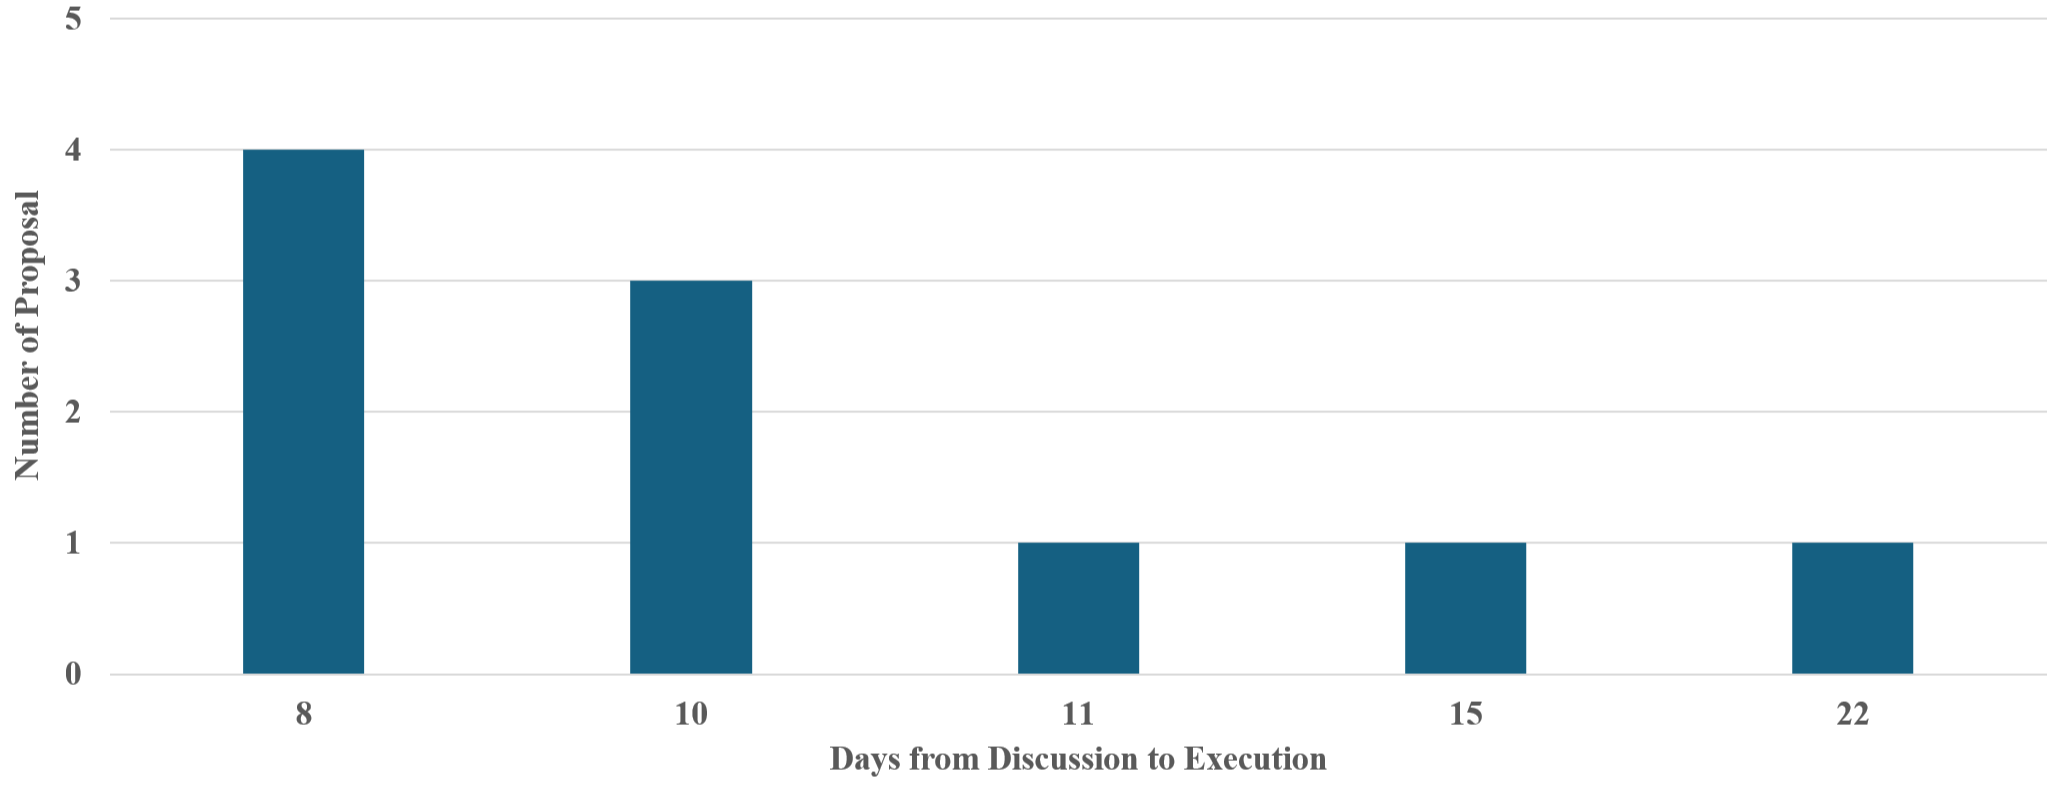
\includegraphics[width=\linewidth]{figure/days_diss_exe.png}}

\end{figure}





\clearpage
\newpage




\begin{landscape}
\begin{figure}[ht!]
\centering
\caption{ Lending Rate}\label{fig:lendingtrate_major}
\caption*{This figure plots the lending rate of lending pools of USDC, DAI, WBTC, and WETH on AAVE and Compound and The Secured Overnight Financing Rate from January 2021 to January 2023.  }

\centering
\subfloat[USD Coin (USDC)]{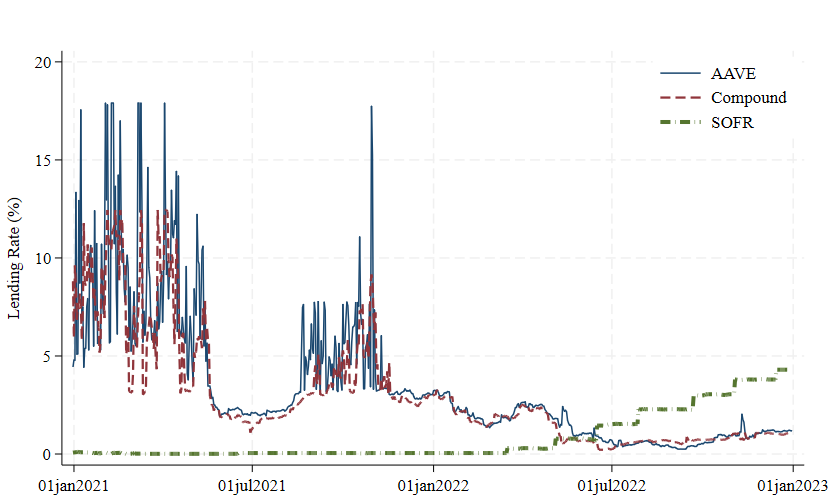
\includegraphics[width=0.45\linewidth]{figure/USDC_LRate.png}}
\subfloat[Dai (DAI)]{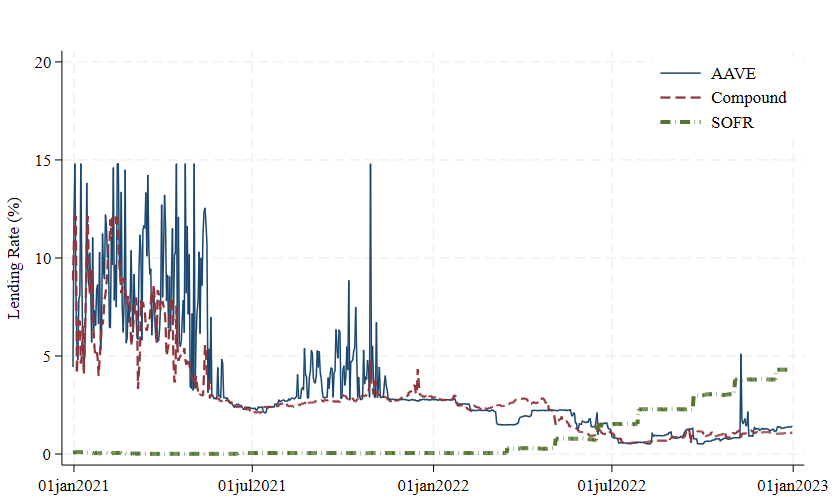
\includegraphics[width=0.45\linewidth]{figure/DAI_LRate.png}}

\subfloat[Wrapped Bitcoin (WBTC)]{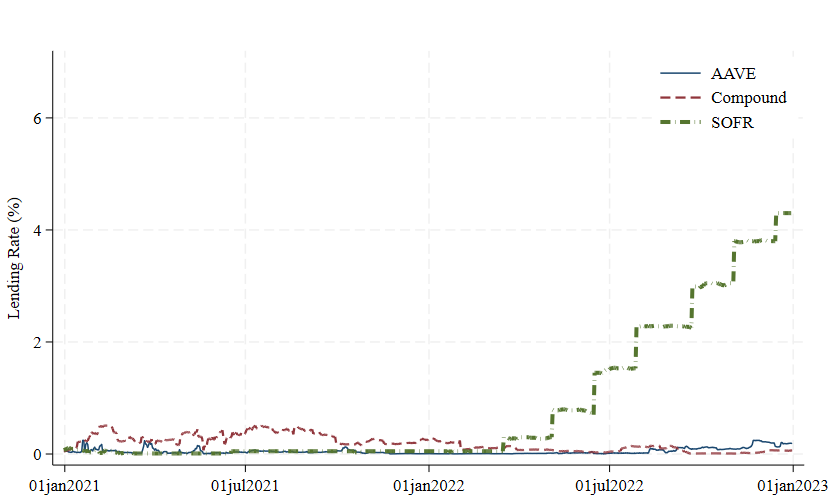
\includegraphics[width=0.45\linewidth]{figure/WBTC_LRate.png}}
\subfloat[Wrapped Ethereum (WETH)]{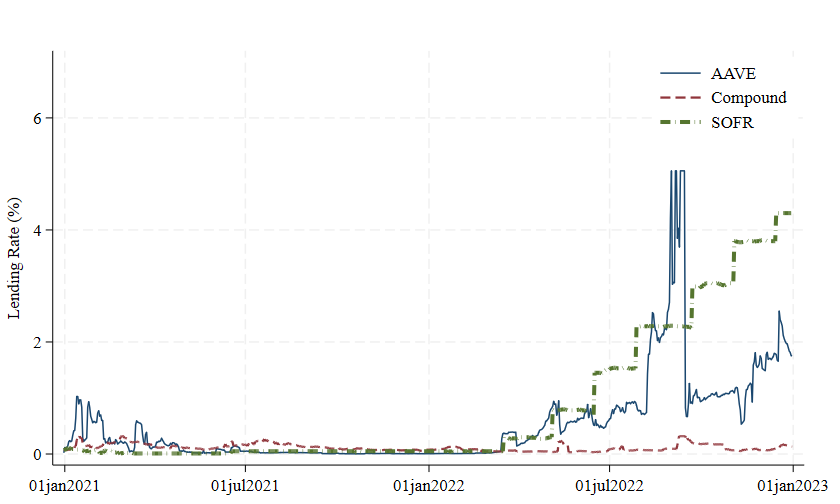
\includegraphics[width=0.45\linewidth]{figure/WETH_LRate.png}}

\end{figure}

\end{landscape}


\clearpage
\newpage
\begin{figure}[ht!]
\centering
\caption{Borrowing and Lending Rate of Other Cryptocurrencies }\label{fig:defi_interestrate_others}
\caption*{This figure plots the lending rate of lending pools other than USDC, DAI, WBTC, and WETH on AAVE and Compound and The Secured Overnight Financing Rate from January 2021 to January 2023. The borrowing (lending) rate is the loan (deposit) amount weighted average of individual cryptocurrencies.}
\subfloat[Borrowing Rate]{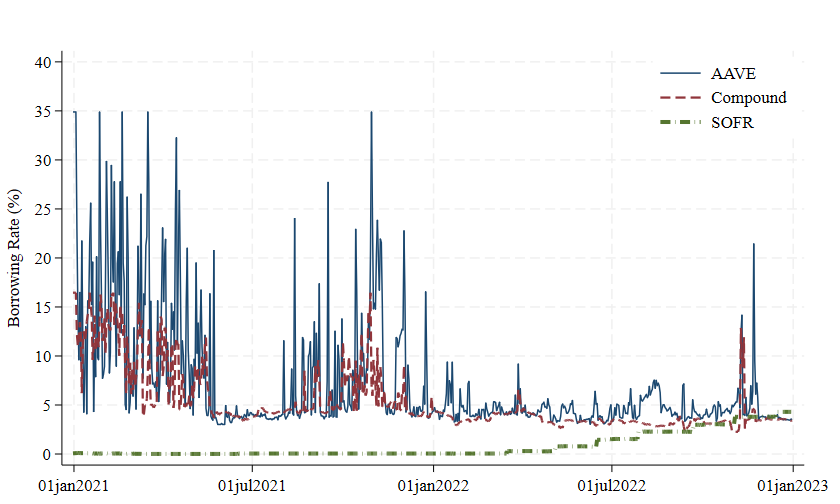
\includegraphics[width=0.9\linewidth]{figure/Others_BRate.png}}


\subfloat[Lending Rate]{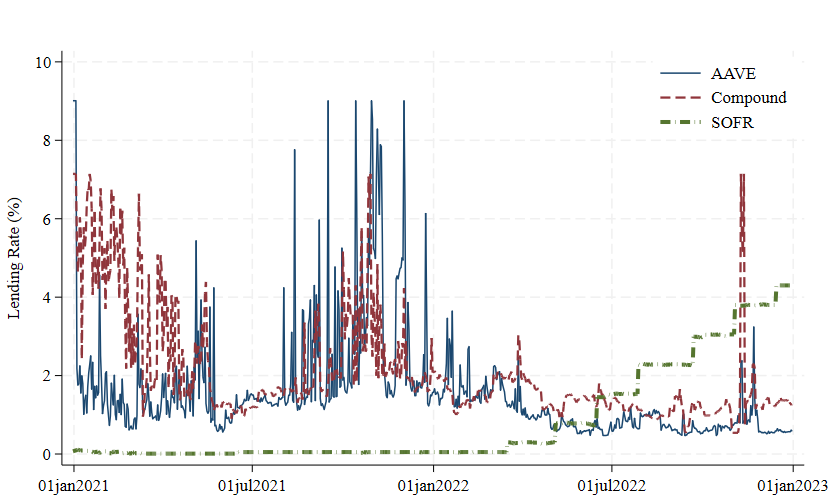
\includegraphics[width=0.9\linewidth]{figure/Others_LRate.png}}

\end{figure}
\clearpage
\newpage


\begin{landscape}
\begin{figure}[ht!]
\centering
\caption{Dynamics of Leverage for Experienced Borrowers}\label{figA:dynamics_lev_experienced}
\caption*{This figure repeats the analysis in Figure \ref{fig:dynamics_lev} using a subsample of experienced borrowers. Experienced borrowers have an account age greater than the median age. Standard errors are clustered at the borrower and week levels. The bars surrounding each coefficient represent the 5\% and 95\% confidence intervals. }

\centering
\subfloat[USD Coin (USDC)]{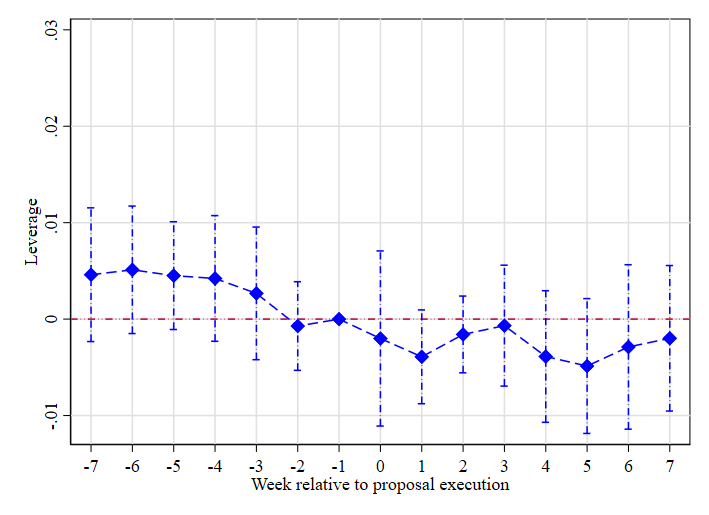
\includegraphics[width=0.4\linewidth]{figure/Heterogeneity/lev_g1_age2.png}}
\subfloat[Dai (DAI)]{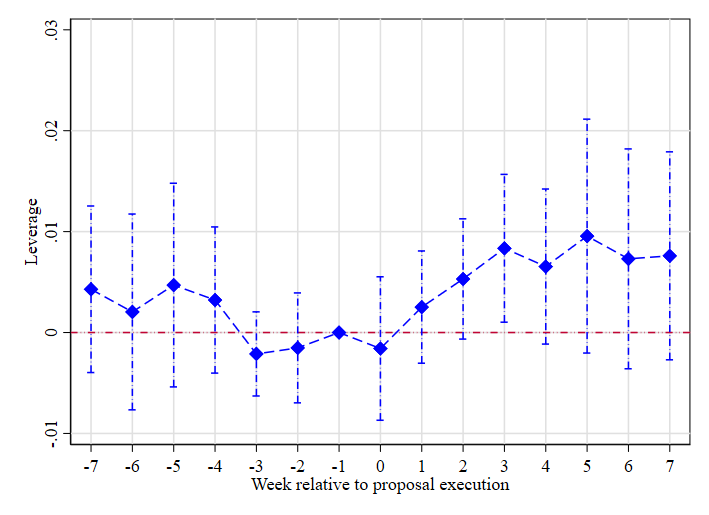
\includegraphics[width=0.4\linewidth]{figure/Heterogeneity/lev_g2_age2.png}}

\subfloat[Wrapped Bitcoin (WBTC)]{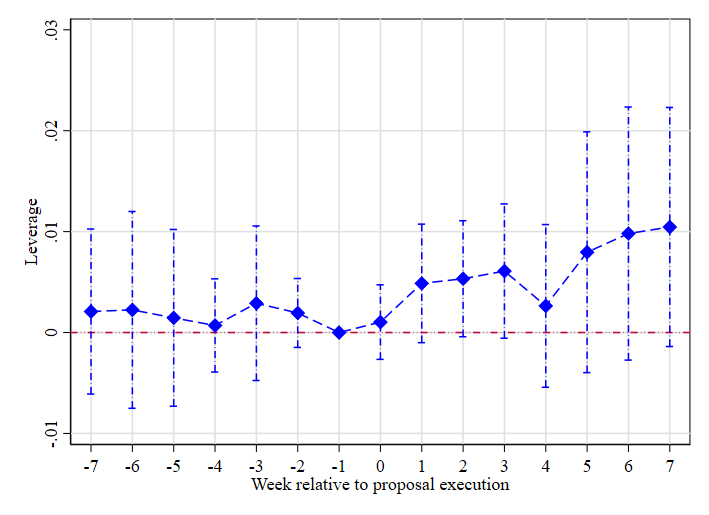
\includegraphics[width=0.4\linewidth]{figure/Heterogeneity/lev_g3_age3.png}}
\subfloat[Wrapped Ethereum (WETH)]{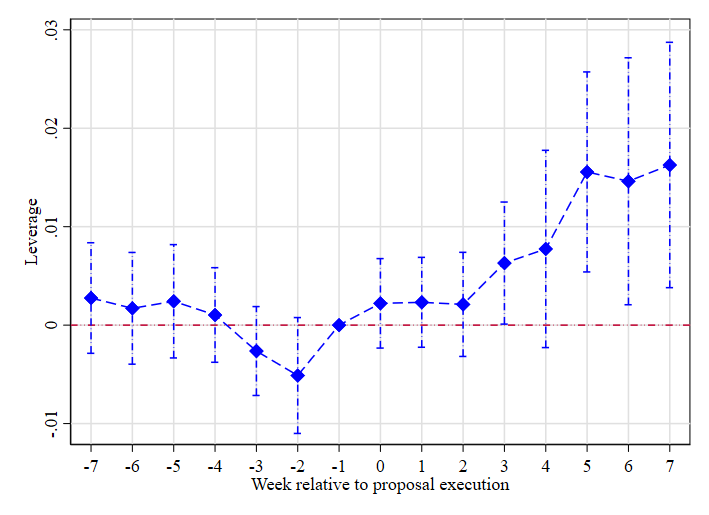
\includegraphics[width=0.4\linewidth]{figure/Heterogeneity/lev_g4_age4.png}}


\end{figure}

\end{landscape}

\clearpage
\newpage

%%%%%%%%%%%% Tables %%%%%%%%%%%%%%%
\clearpage
\newpage
%\setlength{\tabcolsep}{1pt}
    

\begin{table}[ht!]
\small 
\caption{Lending Pools on AAVE and Compound}\label{tabA:lendingpools}
\caption*{This table presents a summary of all lending pools on AAVE (Panel A) and Compound (Panel B). The information includes the names of the lending pools, symbols of lending pools, and whether users can borrow from or use deposits in lending pools as collateral in January 2023.   }

\centering
\def\sym#1{\ifmmode^{#1}\else\(^{#1}\)\fi}

\begin{tabular*}{\linewidth}{@{\extracolsep{\fill}}lllcc}
    \toprule
    Number & Pool Name & Pool Symbol & Can Borrow From? & Can Use as Collateral? \\
    \midrule
    \multicolumn{5}{c}{Panel A: AAVE} \\
    \midrule
    AAVE-1 & TrueUSD & TUSD  & Yes   & Yes \\
    AAVE-2 & Rai Reflex Index & RAI   & \multicolumn{2}{c}{Closed} \\
    AAVE-3 & Gemini dollar & GUSD  & No    & Yes \\
    AAVE-4 & yearn.finance & YFI   & \multicolumn{2}{c}{Closed} \\
    AAVE-5 & Basic Attention Token & BAT   & \multicolumn{2}{c}{Closed} \\
    AAVE-6 & Decentraland MANA & MANA  & \multicolumn{2}{c}{Closed} \\
    AAVE-7 & 1INCH Token & 1INCH & No    & Yes \\
    AAVE-8 & DefiPulse Index & DPI   & No    & Yes \\
    AAVE-9 & Uniswap & UNI   & No    & Yes \\
    AAVE-10 & Wrapped BTC & WBTC  & Yes   & Yes \\
    AAVE-11 & Republic Token & REN   & \multicolumn{2}{c}{Closed} \\
    AAVE-12 & Convex Token & CVX   & \multicolumn{2}{c}{Closed} \\
    AAVE-13 & Binance USD & BUSD  & Yes   & No \\
    AAVE-14 & ChainLink Token & LINK  & No    & Yes \\
    AAVE-15 & Synth sUSD & sUSD  & No    & Yes \\
    AAVE-16 & LUSD Stablecoin & LUSD  & No    & Yes \\
    AAVE-17 & Dai Stablecoin & DAI   & Yes   & Yes \\
    AAVE-18 & Aave Token & AAVE  & No    & Yes \\
    AAVE-19 & Frax  & FRAX  & Yes   & No \\
    AAVE-20 & SushiBar & xSUSHI & \multicolumn{2}{c}{Closed} \\
    AAVE-21 & Paxos Standard & PAX   & No    & Yes \\
    AAVE-22 & Fei USD & FEI   & \multicolumn{2}{c}{Closed} \\
    AAVE-23 & Maker & MKR   & No    & Yes \\
    AAVE-24 & USD Coin & USDC  & Yes   & Yes \\
    AAVE-25 & UST (Wormhole) & UST   & \multicolumn{2}{c}{Closed} \\
    AAVE-26 & Liquid staked Ether 2.0 & stETH & No    & Yes \\
    AAVE-27 & Balancer & BAL   & \multicolumn{2}{c}{Closed} \\
    AAVE-28 & Synthetix Network Token & SNX   & No    & Yes \\
    AAVE-29 & Wrapped Ether & WETH  & Yes   & Yes \\
    AAVE-30 & Ethereum Name Service & ENS   & No    & Yes \\
    AAVE-31 & Ampleforth & AMPL  & \multicolumn{2}{c}{Closed} \\
    AAVE-32 & renFIL & renFIL & \multicolumn{2}{c}{Closed} \\
    AAVE-33 & Curve DAO Token & CRV   & No    & Yes \\
    AAVE-34 & Tether USD & USDT  & Yes   & No \\
    AAVE-35 & Kyber Network Crystal & KNC   & Yes   & Yes \\
    AAVE-36 & 0x Protocol Token & ZRX   & \multicolumn{2}{c}{Closed} \\
    AAVE-37 & Enjin Coin & ENJ   & \multicolumn{2}{c}{Closed} \\
    \bottomrule
        \\ \multicolumn{5}{r}{\textit{(continued on next page)}}\\
          \end{tabular*} 

\end{table}%

\clearpage
\newpage


\begin{table}[ht!]
\small
\centering
\caption*{Table \ref*{tabA:lendingpools} -- Continued from previous page}

\begin{tabular*}{\linewidth}{@{\extracolsep{\fill}}lllcc}
    \toprule
    Number & Pool Name & Pool Symbol & Can Borrow From? & Can Use as Collateral? \\
    \midrule
    \multicolumn{5}{c}{Panel B: Compound} \\
    \midrule
    COMP-1 & Aave Token & AAVE  & Yes   & Yes \\
    COMP-2 & Basic Attention Token & BAT   & Yes   & Yes \\
    COMP-3 & Compound & COMP  & Yes   & Yes \\
    COMP-4 & Dai Stablecoin & DAI   & Yes   & Yes \\
    COMP-5 & Dai Stablecoin v1.0 & DAI   & \multicolumn{2}{c}{Closed} \\
    COMP-6 & Fei USD & FEI   & \multicolumn{2}{c}{Closed} \\
    COMP-7 & ChainLink Token & LINK  & Yes   & Yes \\
    COMP-8 & Maker & MKR   & Yes   & Yes \\
    COMP-9 & Reputation & REP   & \multicolumn{2}{c}{Closed} \\
    COMP-10 & SushiToken & SUSHI & Yes   & Yes \\
    COMP-11 & TrueUSD & TUSD  & Yes   & No \\
    COMP-12 & Uniswap & UNI   & Yes   & Yes \\
    COMP-13 & USD Coin & USDC  & Yes   & Yes \\
    COMP-14 & Pax Dollar & USDP  & Yes   & No \\
    COMP-15 & Tether USD & USDT  & Yes   & No \\
    COMP-16 & Wrapped BTC & WBTC  & Yes   & Yes \\
    COMP-17 & Wrapped Ether & WETH  & Yes   & Yes \\
    COMP-18 & yearn.finance & YFI   & Yes   & Yes \\
    COMP-19 & 0x Protocol Token & ZRX   & Yes   & Yes \\
    \bottomrule
          \end{tabular*} 
 

\end{table}

\clearpage
\newpage
%\setlength{\tabcolsep}{1pt}
    

\begin{table}[ht!]
%\footnotesize 
\caption{Summary Statistics of Borrowing and Lending Positions by Events}\label{tabA:sumstat_bypool}
\caption*{This table presents summary statistics of borrowing and lending positions for each event. Table \ref{tab:proposal_margin} lists the proposal ID and the treated and control pools in each event. $Deposit$ is the US dollar amount (in thousands) of the deposit balance in the treated or control pool. $TotalDeposit$ is the aggregated deposit balance in thousands, calculated by summing the US dollar amounts across all lending positions on the platform. $TotalBorrow$ is the aggregated loan balance in thousands, calculated by summing the dollar amounts across all borrowing positions on the platform. $Leverage$ is the ratio of the total market value of assets ($TotalDeposit+Total Borrow$) and the equity value ($Total Deposit$). Panel A presents the summary statistics of borrowing and lending positions, and Panel B compares the borrowing and lending positions between the treatment and control groups, using observations at the end of the week before the proposal discussion. All financial variables are winsorized at the 1$^{st}$ and 99$^{th}$ percentiles. }

\centering
\def\sym#1{\ifmmode^{#1}\else\(^{#1}\)\fi}






\end{table}%

\clearpage
\newpage
%\setlength{\tabcolsep}{1pt}
    

\begin{table}[ht!]
\footnotesize 
% \caption*{ }

\centering
\def\sym#1{\ifmmode^{#1}\else\(^{#1}\)\fi}


\begin{tabular*}{\linewidth}{@{\extracolsep{\fill}}lcccccc }
    \multicolumn{7}{c}{Appendix Table \ref{tabA:sumstat_bypool} - Proposal AAVE-69 (Treated: AAVE-USDC, Control: COMP-USDC)} \\
    \toprule
     Variable  &N & Mean & SD & P25 & Median & P75 \\
     \midrule
    \multicolumn{7}{c}{Panel A: Summary Statistics on Borrower Account-Week Data} \\
    \midrule
    Deposit (\$, thousand) & 15,740 & 232.65 & 1,059.69 & 0.50  & 3.33  & 45.44 \\
          &       &       &       &       &       &  \\
    TotalDeposit (\$, thousand) & 15,740 & 419.32 & 1,697.89 & 1.59  & 13.74 & 129.59 \\
          &       &       &       &       &       &  \\
    TotalBorrow (\$, thousand) & 15,740 & 149.62 & 607.14 & 0.53  & 5.08  & 49.94 \\
          &       &       &       &       &       &  \\
    Leverage & 15,193 & 1.49  & 0.23  & 1.34  & 1.52  & 1.67 \\
    \midrule
        \multicolumn{7}{c}{Panel B: Differences across the Treated and Control Borrowers} \\
\midrule
          & \multicolumn{2}{c}{Control} &       & \multicolumn{2}{c}{Treated} &  \\
\cmidrule{2-3}\cmidrule{5-6}          & N & Mean &       & N & Mean & Difference \\
\cmidrule{2-3}\cmidrule{5-6}          & (1) & (2) &       & (3) & (4) & (4)-(2) \\
\cmidrule{2-7}    Deposit (\$, thousand) & 318   & 371.28 &       & 734   & 246.44 & -124.84 \\
          &       &       &       &       &       & (78.79) \\
    TotalDeposit (\$, thousand) & 318   & 650.25 &       & 734   & 451.13 & -199.12 \\
          &       &       &       &       &       & (126.68) \\
    TotalBorrow (\$, thousand) & 318   & 212.19 &       & 734   & 180.31 & -31.88 \\
          &       &       &       &       &       & (47.16) \\
    Leverage & 318   & 1.47  &       & 734   & 1.49  & 0.02 \\
          &       &       &       &       &       & (0.02) \\
    \bottomrule
              &       &       &       &       &       &  \\
      \multicolumn{7}{c}{Appendix Table \ref{tabA:sumstat_bypool} - Proposal AAVE-92 (Treated: AAVE-DAI, Control: COMP-DAI)} \\
      \toprule
     Variable  &N & Mean & SD & P25 & Median & P75 \\
     \midrule
    \multicolumn{7}{c}{Panel A: Summary Statistics on Borrower Account-Week Data} \\
    \midrule
    Deposit (\$, thousand) & 8,541 & 71.94 & 540.88 & 0.29  & 1.12  & 9.72 \\
          &       &       &       &       &       &  \\
    TotalDeposit (\$, thousand) & 8,541 & 157.70 & 940.19 & 0.62  & 3.56  & 33.53 \\
          &       &       &       &       &       &  \\
    TotalBorrow (\$, thousand) & 8,541 & 61.37 & 358.37 & 0.25  & 1.44  & 11.44 \\
          &       &       &       &       &       &  \\
    Leverage & 8,257 & 1.49  & 0.21  & 1.36  & 1.53  & 1.66 \\
    \midrule
        \multicolumn{7}{c}{Panel B: Differences across the Treated and Control Borrowers} \\
\midrule
          & \multicolumn{2}{c}{Control} &       & \multicolumn{2}{c}{Treated} &  \\
\cmidrule{2-3}\cmidrule{5-6}          & N & Mean &       & N & Mean & Difference \\
\cmidrule{2-3}\cmidrule{5-6}          & (1) & (2) &       & (3) & (4) & (4)-(2) \\
\cmidrule{2-7}    Deposit (\$, thousand) & 247   & 70.61 &       & 330   & 108.18 & 37.57 \\
          &       &       &       &       &       & (50.61) \\
    TotalDeposit (\$, thousand) & 247   & 105.88 &       & 330   & 264.95 & 159.07* \\
          &       &       &       &       &       & (93.61) \\
    TotalBorrow (\$, thousand) & 247   & 42.36 &       & 330   & 99.26 & 56.90 \\
          &       &       &       &       &       & (37.42) \\
    Leverage & 247   & 1.50  &       & 330   & 1.47  & -0.03* \\
          &       &       &       &       &       & (0.02) \\
    \bottomrule
          \end{tabular*} 



 \end{table}%

% \clearpage
% \newpage
%\setlength{\tabcolsep}{1pt}
    

% \begin{table}[ht!]
% \footnotesize 
% \caption*{Appendix Table \ref{tabA:sumstat_bypool} - Proposal AAVE-92 (Treated: AAVE-DAI, Control: COMP-DAI)}

% \centering
% \def\sym#1{\ifmmode^{#1}\else\(^{#1}\)\fi}


% \begin{tabular*}{\linewidth}{@{\extracolsep{\fill}}lcccccc }
%     \toprule
%      Variable  &N & Mean & SD & P25 & Median & P75 \\
%      \midrule
%     \multicolumn{7}{c}{Panel A: Summary Statistics on Borrower Account-Week Data} \\
%     \midrule
%     Deposit (\$, thousand) & 8,541 & 71.94 & 540.88 & 0.29  & 1.12  & 9.72 \\
%           &       &       &       &       &       &  \\
%     TotalDeposit (\$, thousand) & 8,541 & 157.70 & 940.19 & 0.62  & 3.56  & 33.53 \\
%           &       &       &       &       &       &  \\
%     TotalBorrow (\$, thousand) & 8,541 & 61.37 & 358.37 & 0.25  & 1.44  & 11.44 \\
%           &       &       &       &       &       &  \\
%     Leverage & 8,257 & 1.49  & 0.21  & 1.36  & 1.53  & 1.66 \\
%     \midrule
%         \multicolumn{7}{c}{Panel B: Differences across the Treated and Control Borrowers} \\
% \midrule
%           & \multicolumn{2}{c}{Control} &       & \multicolumn{2}{c}{Treated} &  \\
% \cmidrule{2-3}\cmidrule{5-6}          & N & Mean &       & N & Mean & Difference \\
% \cmidrule{2-3}\cmidrule{5-6}          & (1) & (2) &       & (3) & (4) & (4)-(2) \\
% \cmidrule{2-7}    Deposit (\$, thousand) & 247   & 70.61 &       & 330   & 108.18 & 37.57 \\
%           &       &       &       &       &       & (50.61) \\
%     TotalDeposit (\$, thousand) & 247   & 105.88 &       & 330   & 264.95 & 159.07* \\
%           &       &       &       &       &       & (93.61) \\
%     TotalBorrow (\$, thousand) & 247   & 42.36 &       & 330   & 99.26 & 56.90 \\
%           &       &       &       &       &       & (37.42) \\
%     Leverage & 247   & 1.50  &       & 330   & 1.47  & -0.03* \\
%           &       &       &       &       &       & (0.02) \\
%     \bottomrule
%           \end{tabular*} 



% \end{table}%

\clearpage
\newpage
%\setlength{\tabcolsep}{1pt}
    

\begin{table}[ht!]
\footnotesize 
% \caption*{Appendix Table \ref{tabA:sumstat_bypool} - Proposal AAVE-94 (Treated: AAVE-WBTC, Control: COMP-WBTC)}

\centering
\def\sym#1{\ifmmode^{#1}\else\(^{#1}\)\fi}


\begin{tabular*}{\linewidth}{@{\extracolsep{\fill}}lcccccc }
      \multicolumn{7}{c}{Appendix Table \ref{tabA:sumstat_bypool} - Proposal AAVE-94 (Treated: AAVE-WBTC, Control: COMP-WBTC)} \\
    \toprule
     Variable  &N & Mean & SD & P25 & Median & P75 \\
     \midrule
    \multicolumn{7}{c}{Panel A: Summary Statistics on Borrower Account-Week Data} \\
    \midrule
    Deposit (\$, thousand) & 24,825 & 290.66 & 1,137.83 & 2.38  & 19.17 & 85.81 \\
          &       &       &       &       &       &  \\
    TotalDeposit (\$, thousand) & 24,825 & 523.01 & 1,879.95 & 7.24  & 39.94 & 190.05 \\
          &       &       &       &       &       &  \\
    TotalBorrow (\$, thousand) & 24,825 & 194.81 & 696.48 & 2.86  & 14.56 & 70.08 \\
          &       &       &       &       &       &  \\
    Leverage & 24,086 & 1.43  & 0.17  & 1.32  & 1.44  & 1.55 \\
    \midrule
        \multicolumn{7}{c}{Panel B: Differences across the Treated and Control Borrowers} \\
\midrule
          & \multicolumn{2}{c}{Control} &       & \multicolumn{2}{c}{Treated} &  \\
\cmidrule{2-3}\cmidrule{5-6}          & N & Mean &       & N & Mean & Difference \\
\cmidrule{2-3}\cmidrule{5-6}          & (1) & (2) &       & (3) & (4) & (4)-(2) \\
\cmidrule{2-7}    Deposit (\$, thousand) & 531   & 418.46 &       & 1,124 & 334.95 & -83.51 \\
          &       &       &       &       &       & (68.41) \\
    TotalDeposit (\$, thousand) & 531   & 778.19 &       & 1,124 & 573.76 & -204.43* \\
          &       &       &       &       &       & (111.89) \\
    TotalBorrow (\$, thousand) & 531   & 257.95 &       & 1,124 & 201.75 & -56.20 \\
          &       &       &       &       &       & (39.62) \\
    Leverage & 531   & 1.37  &       & 1,124 & 1.38  & 0.01** \\
          &       &       &       &       &       & (0.00) \\
    \bottomrule
          &       &       &       &       &       &  \\
      \multicolumn{7}{c}{Appendix Table \ref{tabA:sumstat_bypool} - Proposal AAVE-102 (Treated: AAVE-USDC, Control: COMP-USDC)} \\
  \toprule
     Variable  &N & Mean & SD & P25 & Median & P75 \\
     \midrule
    \multicolumn{7}{c}{Panel A: Summary Statistics on Borrower Account-Week Data} \\
    \midrule
    Deposit (\$, thousand) & 19,968 & 258.89 & 1,105.99 & 0.54  & 5.84  & 53.90 \\
          &       &       &       &       &       &  \\
    TotalDeposit (\$, thousand) & 19,968 & 393.31 & 1,633.30 & 1.51  & 16.03 & 116.95 \\
          &       &       &       &       &       &  \\
    TotalBorrow (\$, thousand) & 19,968 & 163.76 & 662.06 & 0.54  & 6.09  & 50.03 \\
          &       &       &       &       &       &  \\
    Leverage & 19,138 & 1.52  & 0.24  & 1.36  & 1.55  & 1.71 \\
    \midrule
        \multicolumn{7}{c}{Panel B: Differences across the Treated and Control Borrowers} \\
\midrule
          & \multicolumn{2}{c}{Control} &       & \multicolumn{2}{c}{Treated} &  \\
\cmidrule{2-3}\cmidrule{5-6}          & N & Mean &       & N & Mean & Difference \\
\cmidrule{2-3}\cmidrule{5-6}          & (1) & (2) &       & (3) & (4) & (4)-(2) \\
\cmidrule{2-7}    Deposit (\$, thousand) & 295   & 341.63 &       & 1,025 & 319.37 & -22.26 \\
          &       &       &       &       &       & (84.07) \\
    TotalDeposit (\$, thousand) & 295   & 471.89 &       & 1,025 & 453.24 & -18.65 \\
          &       &       &       &       &       & (119.96) \\
    TotalBorrow (\$, thousand) & 295   & 144.00 &       & 1,025 & 185.34 & 41.34 \\
          &       &       &       &       &       & (45.21) \\
    Leverage & 295   & 1.46  &       & 1,025 & 1.53  & 0.07*** \\
          &       &       &       &       &       & (0.02) \\
    \bottomrule
    
          \end{tabular*} 



\end{table}%


% \clearpage
% \newpage
% \begin{table}[ht!]
% %\footnotesize 
% \caption*{Appendix Table \ref{tabA:sumstat_bypool} - Proposal AAVE-102 (Treated: AAVE-USDC, Control: COMP-USDC)}

% \centering
% \def\sym#1{\ifmmode^{#1}\else\(^{#1}\)\fi}


% \begin{tabular*}{\linewidth}{@{\extracolsep{\fill}}lcccccc }
%     \toprule
%      Variable  &N & Mean & SD & P25 & Median & P75 \\
%      \midrule
%     \multicolumn{7}{c}{Panel A: Summary Statistics on Borrower Account-Week Data} \\
%     \midrule
%     Deposit (\$, thousand) & 19,968 & 258.89 & 1105.99 & 0.54  & 5.84  & 53.90 \\
%           &       &       &       &       &       &  \\
%     TotalDeposit (\$, thousand) & 19,968 & 393.31 & 1633.30 & 1.51  & 16.03 & 116.95 \\
%           &       &       &       &       &       &  \\
%     TotalBorrow (\$, thousand) & 19,968 & 163.76 & 662.06 & 0.54  & 6.09  & 50.03 \\
%           &       &       &       &       &       &  \\
%     Leverage & 19,138 & 1.52  & 0.24  & 1.36  & 1.55  & 1.71 \\
%     \midrule
%         \multicolumn{7}{c}{Panel B: Differences across the Treated and Control Borrowers} \\
% \midrule
%           & \multicolumn{2}{c}{Control} &       & \multicolumn{2}{c}{Treated} &  \\
% \cmidrule{2-3}\cmidrule{5-6}          & N & Mean &       & N & Mean & Difference \\
% \cmidrule{2-3}\cmidrule{5-6}          & (1) & (2) &       & (3) & (4) & (4)-(2) \\
% \cmidrule{2-7}    Deposit (\$, thousand) & 295   & 341.63 &       & 1,025 & 319.37 & -22.26 \\
%           &       &       &       &       &       & (84.07) \\
%     TotalDeposit (\$, thousand) & 295   & 471.89 &       & 1,025 & 453.24 & -18.65 \\
%           &       &       &       &       &       & (119.96) \\
%     TotalBorrow (\$, thousand) & 295   & 144.00 &       & 1,025 & 185.34 & 41.34 \\
%           &       &       &       &       &       & (45.21) \\
%     Leverage & 295   & 1.46  &       & 1,025 & 1.53  & 0.07*** \\
%           &       &       &       &       &       & (0.02) \\
%     \bottomrule
%           \end{tabular*} 



% \end{table}%

\clearpage
\newpage
\begin{table}[ht!]
\footnotesize 
% \caption*{Appendix Table \ref{tabA:sumstat_bypool} - Proposal AAVE-102 (Treated: AAVE-WETH, Control: COMP-WETH)}

\centering
\def\sym#1{\ifmmode^{#1}\else\(^{#1}\)\fi}


\begin{tabular*}{\linewidth}{@{\extracolsep{\fill}}lcccccc }
      \multicolumn{7}{c}{Appendix Table \ref{tabA:sumstat_bypool} - Proposal AAVE-102 (Treated: AAVE-WETH, Control: COMP-WETH)} \\
    \toprule
     Variable  &N & Mean & SD & P25 & Median & P75 \\
     \midrule
    \multicolumn{7}{c}{Panel A: Summary Statistics on Borrower Account-Week Data} \\
    \midrule
    Deposit (\$, thousand) & 66,360 & 152.10 & 787.66 & 0.78  & 5.37  & 35.12 \\
          &       &       &       &       &       &  \\
    TotalDeposit (\$, thousand) & 66,360 & 251.52 & 1,247.01 & 1.35  & 9.83  & 61.36 \\
          &       &       &       &       &       &  \\
    TotalBorrow (\$, thousand) & 66,360 & 95.79 & 474.79 & 0.52  & 3.71  & 24.46 \\
          &       &       &       &       &       &  \\
    Leverage & 64,861 & 1.46  & 0.20  & 1.33  & 1.47  & 1.60 \\
    \midrule
        \multicolumn{7}{c}{Panel B: Differences across the Treated and Control Borrowers} \\
\midrule
          & \multicolumn{2}{c}{Control} &       & \multicolumn{2}{c}{Treated} &  \\
\cmidrule{2-3}\cmidrule{5-6}          & N & Mean &       & N & Mean & Difference \\
\cmidrule{2-3}\cmidrule{5-6}          & (1) & (2) &       & (3) & (4) & (4)-(2) \\
\cmidrule{2-7}    Deposit (\$, thousand) & 1,263 & 181.64 &       & 3,137 & 149.43 & -32.21 \\
          &       &       &       &       &       & (26.58) \\
    TotalDeposit (\$, thousand) & 1,263 & 282.63 &       & 3,137 & 249.67 & -32.96 \\
          &       &       &       &       &       & (42.08) \\
    TotalBorrow (\$, thousand) & 1,263 & 107.20 &       & 3,137 & 99.55 & -7.65 \\
          &       &       &       &       &       & (16.54) \\
    Leverage & 1,263 & 1.46  &       & 3,137 & 1.46  & 0.00 \\
          &       &       &       &       &       & (0.01) \\
    \bottomrule

              &       &       &       &       &       &  \\
      \multicolumn{7}{c}{Appendix Table \ref{tabA:sumstat_bypool} - Proposal AAVE-108 (Treated: AAVE-WBTC, Control: COMP-WBTC)} \\
         \toprule
     Variable  &N & Mean & SD & P25 & Median & P75 \\
     \midrule
    \multicolumn{7}{c}{Panel A: Summary Statistics on Borrower Account-Week Data} \\
    \midrule
    Deposit (\$, thousand) & 25,944 & 270.15 & 1,096.22 & 1.98  & 16.36 & 76.11 \\
          &       &       &       &       &       &  \\
    TotalDeposit (\$, thousand) & 25,944 & 476.90 & 1,760.83 & 6.60  & 37.01 & 167.35 \\
          &       &       &       &       &       &  \\
    TotalBorrow (\$, thousand) & 25,944 & 189.29 & 685.59 & 2.50  & 13.54 & 65.44 \\
          &       &       &       &       &       &  \\
    Leverage & 25,169 & 1.45  & 0.18  & 1.33  & 1.47  & 1.58 \\
    \midrule
        \multicolumn{7}{c}{Panel B: Differences across the Treated and Control Borrowers} \\
\midrule
          & \multicolumn{2}{c}{Control} &       & \multicolumn{2}{c}{Treated} &  \\
\cmidrule{2-3}\cmidrule{5-6}          & N & Mean &       & N & Mean & Difference \\
\cmidrule{2-3}\cmidrule{5-6}          & (1) & (2) &       & (3) & (4) & (4)-(2) \\
\cmidrule{2-7}    Deposit (\$, thousand) & 509   & 348.42 &       & 1,220 & 270.17 & -78.25 \\
          &       &       &       &       &       & (59.50) \\
    TotalDeposit (\$, thousand) & 509   & 588.22 &       & 1,220 & 452.52 & -135.70 \\
          &       &       &       &       &       & (93.89) \\
    TotalBorrow (\$, thousand) & 509   & 227.95 &       & 1,220 & 178.60 & -49.35 \\
          &       &       &       &       &       & (35.86) \\
    Leverage & 509   & 1.46  &       & 1,220 & 1.45  & 0.01 \\
          &       &       &       &       &       & (0.01) \\
    \bottomrule
          \end{tabular*} 



\end{table}%

% \clearpage
% \newpage
% \begin{table}[ht!]
% %\footnotesize 
% \caption*{Appendix Table \ref{tabA:sumstat_bypool} - Proposal AAVE-108 (Treated: AAVE-WBTC, Control: COMP-WBTC)}

% \centering
% \def\sym#1{\ifmmode^{#1}\else\(^{#1}\)\fi}


% \begin{tabular*}{\linewidth}{@{\extracolsep{\fill}}lcccccc }
%     \toprule
%      Variable  &N & Mean & SD & P25 & Median & P75 \\
%      \midrule
%     \multicolumn{7}{c}{Panel A: Summary Statistics on Borrower Account-Week Data} \\
%     \midrule
%     Deposit (\$, thousand) & 25,944 & 270.15 & 1096.22 & 1.98  & 16.36 & 76.11 \\
%           &       &       &       &       &       &  \\
%     TotalDeposit (\$, thousand) & 25,944 & 476.90 & 1760.83 & 6.60  & 37.01 & 167.35 \\
%           &       &       &       &       &       &  \\
%     TotalBorrow (\$, thousand) & 25,944 & 189.29 & 685.59 & 2.50  & 13.54 & 65.44 \\
%           &       &       &       &       &       &  \\
%     Leverage & 25,169 & 1.45  & 0.18  & 1.33  & 1.47  & 1.58 \\
%     \midrule
%         \multicolumn{7}{c}{Panel B: Differences across the Treated and Control Borrowers} \\
% \midrule
%           & \multicolumn{2}{c}{Control} &       & \multicolumn{2}{c}{Treated} &  \\
% \cmidrule{2-3}\cmidrule{5-6}          & N & Mean &       & N & Mean & Difference \\
% \cmidrule{2-3}\cmidrule{5-6}          & (1) & (2) &       & (3) & (4) & (4)-(2) \\
% \cmidrule{2-7}    Deposit (\$, thousand) & 509   & 348.42 &       & 1,220 & 270.17 & -78.25 \\
%           &       &       &       &       &       & (59.50) \\
%     TotalDeposit (\$, thousand) & 509   & 588.22 &       & 1,220 & 452.52 & -135.70 \\
%           &       &       &       &       &       & (93.89) \\
%     TotalBorrow (\$, thousand) & 509   & 227.95 &       & 1,220 & 178.60 & -49.35 \\
%           &       &       &       &       &       & (35.86) \\
%     Leverage & 509   & 1.46  &       & 1,220 & 1.45  & 0.01 \\
%           &       &       &       &       &       & (0.01) \\
%     \bottomrule
%           \end{tabular*} 



% \end{table}%

\clearpage
\newpage
\begin{table}[ht!]
\footnotesize 
% \caption*{Appendix Table \ref{tabA:sumstat_bypool} - Proposal COMP-36 (Treated: COMP-WBTC, Control: AAVE-WBTC)}

\centering
\def\sym#1{\ifmmode^{#1}\else\(^{#1}\)\fi}


\begin{tabular*}{\linewidth}{@{\extracolsep{\fill}}lcccccc }
      \multicolumn{7}{c}{Appendix Table \ref{tabA:sumstat_bypool} - Proposal COMP-36 (Treated: COMP-WBTC, Control: AAVE-WBTC)} \\
      
    \toprule
     Variable  &N & Mean & SD & P25 & Median & P75 \\
     \midrule
    \multicolumn{7}{c}{Panel A: Summary Statistics on Borrower Account-Week Data} \\
    \midrule
    Deposit (\$, thousand) & 16,110 & 382.43 & 1,341.46 & 0.05  & 14.61 & 111.60 \\
          &       &       &       &       &       &  \\
    TotalDeposit (\$, thousand) & 16,110 & 771.81 & 2,361.48 & 5.71  & 56.91 & 320.04 \\
          &       &       &       &       &       &  \\
    TotalBorrow (\$, thousand) & 16,110 & 279.76 & 896.60 & 0.99  & 15.01 & 100.49 \\
          &       &       &       &       &       &  \\
    Leverage & 14,087 & 1.33  & 0.17  & 1.22  & 1.34  & 1.45 \\
    \midrule
        \multicolumn{7}{c}{Panel B: Differences across the Treated and Control Borrowers} \\
\midrule
          & \multicolumn{2}{c}{Control} &       & \multicolumn{2}{c}{Treated} &  \\
\cmidrule{2-3}\cmidrule{5-6}          & N & Mean &       & N & Mean & Difference \\
\cmidrule{2-3}\cmidrule{5-6}          & (1) & (2) &       & (3) & (4) & (4)-(2) \\
\cmidrule{2-7}    Deposit (\$, thousand) & 405   & 239.41 &       & 740   & 632.84 & 393.43*** \\
          &       &       &       &       &       & (88.97) \\
    TotalDeposit (\$, thousand) & 405   & 396.17 &       & 740   & 1,046.41 & 650.24*** \\
          &       &       &       &       &       & (142.83) \\
    TotalBorrow (\$, thousand) & 405   & 149.40 &       & 740   & 341.67 & 192.27*** \\
          &       &       &       &       &       & (52.20) \\
    Leverage & 405   & 1.35  &       & 740   & 1.29  & -0.06*** \\
          &       &       &       &       &       & (0.01) \\
    \bottomrule
              &       &       &       &       &       &  \\
      \multicolumn{7}{c}{Appendix Table \ref{tabA:sumstat_bypool} - Proposal COMP-66 (Treated: COMP-USDC, Control: AAVE-USDC)} \\
       \toprule
     Variable  &N & Mean & SD & P25 & Median & P75 \\
     \midrule
    \multicolumn{7}{c}{Panel A: Summary Statistics on Borrower Account-Week Data} \\
    \midrule
    Deposit (\$, thousand) & 16,383 & 318.85 & 1,322.64 & 0.49  & 3.48  & 40.51 \\
          &       &       &       &       &       &  \\
    TotalDeposit (\$, thousand) & 16,383 & 659.06 & 2,295.55 & 2.25  & 19.97 & 187.18 \\
          &       &       &       &       &       &  \\
    TotalBorrow (\$, thousand) & 16,383 & 254.75 & 901.97 & 0.71  & 6.03  & 60.89 \\
          &       &       &       &       &       &  \\
    Leverage & 15,662 & 1.44  & 0.22  & 1.28  & 1.45  & 1.60 \\
    \midrule
        \multicolumn{7}{c}{Panel B: Differences across the Treated and Control Borrowers} \\
\midrule
          & \multicolumn{2}{c}{Control} &       & \multicolumn{2}{c}{Treated} &  \\
\cmidrule{2-3}\cmidrule{5-6}          & N & Mean &       & N & Mean & Difference \\
\cmidrule{2-3}\cmidrule{5-6}          & (1) & (2) &       & (3) & (4) & (4)-(2) \\
\cmidrule{2-7}    Deposit (\$, thousand) & 688   & 312.82 &       & 414   & 473.14 & 160.32* \\
          &       &       &       &       &       & (87.85) \\
    TotalDeposit (\$, thousand) & 688   & 681.00 &       & 414   & 818.07 & 137.07 \\
          &       &       &       &       &       & (148.10) \\
    TotalBorrow (\$, thousand) & 688   & 255.27 &       & 414   & 322.10 & 66.83 \\
          &       &       &       &       &       & (57.07) \\
    Leverage & 688   & 1.45  &       & 414   & 1.44  & 0.01 \\
          &       &       &       &       &       & (0.01) \\
    \bottomrule
          \end{tabular*} 



\end{table}%

% \clearpage
% \newpage
% \begin{table}[ht!]
% %\footnotesize 
% \caption*{Appendix Table \ref{tabA:sumstat_bypool} - Proposal COMP-66 (Treated: COMP-USDC, Control: AAVE-USDC)}

% \centering
% \def\sym#1{\ifmmode^{#1}\else\(^{#1}\)\fi}


% \begin{tabular*}{\linewidth}{@{\extracolsep{\fill}}lcccccc }
%     \toprule
%      Variable  &N & Mean & SD & P25 & Median & P75 \\
%      \midrule
%     \multicolumn{7}{c}{Panel A: Summary Statistics on Borrower Account-Week Data} \\
%     \midrule
%     Deposit (\$, thousand) & 16,383 & 318.85 & 1322.64 & 0.49  & 3.48  & 40.51 \\
%           &       &       &       &       &       &  \\
%     TotalDeposit (\$, thousand) & 16,383 & 659.06 & 2295.55 & 2.25  & 19.97 & 187.18 \\
%           &       &       &       &       &       &  \\
%     TotalBorrow (\$, thousand) & 16,383 & 254.75 & 901.97 & 0.71  & 6.03  & 60.89 \\
%           &       &       &       &       &       &  \\
%     Leverage & 15,662 & 1.44  & 0.22  & 1.28  & 1.45  & 1.60 \\
%     \midrule
%         \multicolumn{7}{c}{Panel B: Differences across the Treated and Control Borrowers} \\
% \midrule
%           & \multicolumn{2}{c}{Control} &       & \multicolumn{2}{c}{Treated} &  \\
% \cmidrule{2-3}\cmidrule{5-6}          & N & Mean &       & N & Mean & Difference \\
% \cmidrule{2-3}\cmidrule{5-6}          & (1) & (2) &       & (3) & (4) & (4)-(2) \\
% \cmidrule{2-7}    Deposit (\$, thousand) & 688   & 312.82 &       & 414   & 473.14 & 160.32* \\
%           &       &       &       &       &       & (87.85) \\
%     TotalDeposit (\$, thousand) & 688   & 681.00 &       & 414   & 818.07 & 137.07 \\
%           &       &       &       &       &       & (148.10) \\
%     TotalBorrow (\$, thousand) & 688   & 255.27 &       & 414   & 322.10 & 66.83 \\
%           &       &       &       &       &       & (57.07) \\
%     Leverage & 688   & 1.45  &       & 414   & 1.44  & 0.01 \\
%           &       &       &       &       &       & (0.01) \\
%     \bottomrule
%           \end{tabular*} 



% \end{table}%

\clearpage
\newpage
\begin{table}[ht!]
\footnotesize 
% \caption*{Appendix Table \ref{tabA:sumstat_bypool} - Proposal COMP-71 (Treated: COMP-DAI, Control: AAVE-DAI)}

\centering
\def\sym#1{\ifmmode^{#1}\else\(^{#1}\)\fi}


\begin{tabular*}{\linewidth}{@{\extracolsep{\fill}}lcccccc }

      \multicolumn{7}{c}{Appendix Table \ref{tabA:sumstat_bypool} - Proposal COMP-71 (Treated: COMP-DAI, Control: AAVE-DAI)} \\
    \toprule
     Variable  &N & Mean & SD & P25 & Median & P75 \\
     \midrule
    \multicolumn{7}{c}{Panel A: Summary Statistics on Borrower Account-Week Data} \\
    \midrule
    Deposit (\$, thousand) & 10,409 & 98.45 & 659.82 & 0.38  & 1.53  & 13.63 \\
          &       &       &       &       &       &  \\
    TotalDeposit (\$, thousand) & 10,409 & 250.53 & 1,243.26 & 1.22  & 8.64  & 74.73 \\
          &       &       &       &       &       &  \\
    TotalBorrow (\$, thousand) & 10,409 & 101.94 & 531.84 & 0.37  & 2.70  & 23.63 \\
          &       &       &       &       &       &  \\
    Leverage & 10,128 & 1.43  & 0.22  & 1.28  & 1.46  & 1.60 \\
    \midrule
        \multicolumn{7}{c}{Panel B: Differences across the Treated and Control Borrowers} \\
\midrule
          & \multicolumn{2}{c}{Control} &       & \multicolumn{2}{c}{Treated} &  \\
\cmidrule{2-3}\cmidrule{5-6}          & N & Mean &       & N & Mean & Difference \\
\cmidrule{2-3}\cmidrule{5-6}          & (1) & (2) &       & (3) & (4) & (4)-(2) \\
\cmidrule{2-7}    Deposit (\$, thousand) & 347   & 113.54 &       & 346   & 108.64 & -4.90 \\
          &       &       &       &       &       & (54.75) \\
    TotalDeposit (\$, thousand) & 347   & 329.41 &       & 346   & 244.84 & -84.57 \\
          &       &       &       &       &       & (99.93) \\
    TotalBorrow (\$, thousand) & 347   & 136.01 &       & 346   & 93.98 & -42.03 \\
          &       &       &       &       &       & (42.75) \\
    Leverage & 347   & 1.42  &       & 346   & 1.43  & 0.01 \\
          &       &       &       &       &       & (0.02) \\
    \bottomrule
              &       &       &       &       &       &  \\
      \multicolumn{7}{c}{Appendix Table \ref{tabA:sumstat_bypool} - Proposal COMP-71 (Treated: COMP-WETH, Control: AAVE-WETH)} \\
        \toprule
     Variable  &N & Mean & SD & P25 & Median & P75 \\
     \midrule
    \multicolumn{7}{c}{Panel A: Summary Statistics on Borrower Account-Week Data} \\
    \midrule
    Deposit (\$, thousand) & 96,292 & 353.17 & 1,242.78 & 3.92  & 24.32 & 133.69 \\
          &       &       &       &       &       &  \\
    TotalDeposit (\$, thousand) & 96,292 & 532.32 & 1,926.97 & 5.74  & 36.92 & 198.46 \\
          &       &       &       &       &       &  \\
    TotalBorrow (\$, thousand) & 96,292 & 191.22 & 708.57 & 1.50  & 11.00 & 63.22 \\
          &       &       &       &       &       &  \\
              Leverage & 92,413 & 1.37  & 0.19  & 1.24  & 1.36  & 1.51 \\

    \midrule
        \multicolumn{7}{c}{Panel B: Differences across the Treated and Control Borrowers} \\
\midrule
          & \multicolumn{2}{c}{Control} &       & \multicolumn{2}{c}{Treated} &  \\
\cmidrule{2-3}\cmidrule{5-6}          & N & Mean &       & N & Mean & Difference \\
\cmidrule{2-3}\cmidrule{5-6}          & (1) & (2) &       & (3) & (4) & (4)-(2) \\
\cmidrule{2-7}    Deposit (\$, thousand) & 4,184 & 397.45 &       & 2,266 & 507.04 & 109.59*** \\
          &       &       &       &       &       & (35.99) \\
    TotalDeposit (\$, thousand) & 4,184 & 583.10 &       & 2,266 & 773.84 & 190.74*** \\
          &       &       &       &       &       & (55.44) \\
    TotalBorrow (\$, thousand) & 4,184 & 209.79 &       & 2,266 & 235.59 & 25.80 \\
          &       &       &       &       &       & (20.01) \\
    Leverage & 4,184 & 1.35  &       & 2,266 & 1.3   & -0.05*** \\
          &       &       &       &       &       & (0.01) \\
    \bottomrule
          \end{tabular*} 



\end{table}%

% \clearpage
% \newpage
% \begin{table}[ht!]
% %\footnotesize 
% \caption*{Appendix Table \ref{tabA:sumstat_bypool} - Proposal COMP-71 (Treated: COMP-WETH, Control: AAVE-WETH)}

% \centering
% \def\sym#1{\ifmmode^{#1}\else\(^{#1}\)\fi}


% \begin{tabular*}{\linewidth}{@{\extracolsep{\fill}}lcccccc }
%     \toprule
%      Variable  &N & Mean & SD & P25 & Median & P75 \\
%      \midrule
%     \multicolumn{7}{c}{Panel A: Summary Statistics on Borrower Account-Week Data} \\
%     \midrule
%     Deposit (\$, thousand) & 96,292 & 353.17 & 1242.78 & 3.92  & 24.32 & 133.69 \\
%           &       &       &       &       &       &  \\
%     TotalDeposit (\$, thousand) & 96,292 & 532.32 & 1926.97 & 5.74  & 36.92 & 198.46 \\
%           &       &       &       &       &       &  \\
%     TotalBorrow (\$, thousand) & 96,292 & 191.22 & 708.57 & 1.50  & 11.00 & 63.22 \\
%           &       &       &       &       &       &  \\
%               Leverage & 92,413 & 1.37  & 0.19  & 1.24  & 1.36  & 1.51 \\

%     \midrule
%         \multicolumn{7}{c}{Panel B: Differences across the Treated and Control Borrowers} \\
% \midrule
%           & \multicolumn{2}{c}{Control} &       & \multicolumn{2}{c}{Treated} &  \\
% \cmidrule{2-3}\cmidrule{5-6}          & N & Mean &       & N & Mean & Difference \\
% \cmidrule{2-3}\cmidrule{5-6}          & (1) & (2) &       & (3) & (4) & (4)-(2) \\
% \cmidrule{2-7}    Deposit (\$, thousand) & 4,184 & 397.45 &       & 2,266 & 507.04 & 109.59*** \\
%           &       &       &       &       &       & (35.98) \\
%     TotalDeposit (\$, thousand) & 4,184 & 583.10 &       & 2,266 & 773.84 & 190.74*** \\
%           &       &       &       &       &       & (55.44) \\
%     TotalBorrow (\$, thousand) & 4,184 & 209.79 &       & 2,266 & 235.59 & 25.80 \\
%           &       &       &       &       &       & (20.01) \\
%     Leverage & 4,184 & 1.35  &       & 2,266 & 1.3   & -0.05*** \\
%           &       &       &       &       &       & (0.01) \\
%     \bottomrule
%           \end{tabular*} 



% \end{table}%

\clearpage
\newpage
\begin{table}[ht!]
\footnotesize 
% \caption*{Appendix Table \ref{tabA:sumstat_bypool} - Proposal COMP-74 (Treated: COMP-WBTC, Control: AAVE-WBTC)}

\centering
\def\sym#1{\ifmmode^{#1}\else\(^{#1}\)\fi}


\begin{tabular*}{\linewidth}{@{\extracolsep{\fill}}lcccccc }
      \multicolumn{7}{c}{Appendix Table \ref{tabA:sumstat_bypool} - Proposal COMP-74 (Treated: COMP-WBTC, Control: AAVE-WBTC)} \\
    \toprule
     Variable  &N & Mean & SD & P25 & Median & P75 \\
     \midrule
    \multicolumn{7}{c}{Panel A: Summary Statistics on Borrower Account-Week Data} \\
    \midrule
    Deposit (\$, thousand) & 30,246 & 407.88 & 1,310.26 & 5.59  & 39.54 & 167.67 \\
          &       &       &       &       &       &  \\
    TotalDeposit (\$, thousand) & 30,246 & 806.12 & 2,327.02 & 20.37 & 94.73 & 407.23 \\
          &       &       &       &       &       &  \\
    TotalBorrow (\$, thousand) & 30,246 & 303.47 & 873.88 & 6.09  & 32.44 & 149.59 \\
          &       &       &       &       &       &  \\
    Leverage & 29,054 & 1.40  & 0.18  & 1.28  & 1.40  & 1.52 \\
    \midrule
        \multicolumn{7}{c}{Panel B: Differences across the Treated and Control Borrowers} \\
\midrule
          & \multicolumn{2}{c}{Control} &       & \multicolumn{2}{c}{Treated} &  \\
\cmidrule{2-3}\cmidrule{5-6}          & N & Mean &       & N & Mean & Difference \\
\cmidrule{2-3}\cmidrule{5-6}          & (1) & (2) &       & (3) & (4) & (4)-(2) \\
\cmidrule{2-7}    Deposit (\$, thousand) & 1,373 & 366.40 &       & 680   & 602.19 & 235.79*** \\
          &       &       &       &       &       & (63.30) \\
    TotalDeposit (\$, thousand) & 1,373 & 765.86 &       & 680   & 1100.05 & 334.19*** \\
          &       &       &       &       &       & (112.61) \\
    TotalBorrow (\$, thousand) & 1,373 & 300.82 &       & 680   & 399.20 & 98.38** \\
          &       &       &       &       &       & (42.33) \\
    Leverage & 1,373 & 1.43  &       & 680   & 1.37  & -0.06*** \\
          &       &       &       &       &       & (0.01) \\
    \bottomrule
                  &       &       &       &       &       &  \\
      \multicolumn{7}{c}{Appendix Table \ref{tabA:sumstat_bypool} - Proposal COMP-81 (Treated: COMP-WETH, Control: AAVE-WETH)} \\
          \toprule
     Variable  &N & Mean & SD & P25 & Median & P75 \\
     \midrule
    \multicolumn{7}{c}{Panel A: Summary Statistics on Borrower Account-Week Data} \\
    \midrule
    Deposit (\$, thousand) & 95,427 & 284.94 & 1,103.01 & 2.62  & 16.75 & 98.50 \\
          &       &       &       &       &       &  \\
    TotalDeposit (\$, thousand) & 95,427 & 428.40 & 1,699.13 & 3.91  & 25.63 & 146.37 \\
          &       &       &       &       &       &  \\
    TotalBorrow (\$, thousand) & 95,427 & 162.43 & 636.92 & 1.35  & 9.57  & 53.08 \\
          &       &       &       &       &       &  \\
    Leverage & 91,636 & 1.44  & 0.21  & 1.29  & 1.44  & 1.59 \\
    \midrule
        \multicolumn{7}{c}{Panel B: Differences across the Treated and Control Borrowers} \\
\midrule
          & \multicolumn{2}{c}{Control} &       & \multicolumn{2}{c}{Treated} &  \\
\cmidrule{2-3}\cmidrule{5-6}          & N & Mean &       & N & Mean & Difference \\
\cmidrule{2-3}\cmidrule{5-6}          & (1) & (2) &       & (3) & (4) & (4)-(2) \\
\cmidrule{2-7}    Deposit (\$, thousand) & 4,209 & 320.73 &       & 2,168 & 408.19 & 87.46*** \\
          &       &       &       &       &       & (32.25) \\
    TotalDeposit (\$, thousand) & 4,209 & 458.47 &       & 2,168 & 606.32 & 147.85*** \\
          &       &       &       &       &       & (48.99) \\
    TotalBorrow (\$, thousand) & 4,209 & 188.85 &       & 2,168 & 215.72 & 26.87 \\
          &       &       &       &       &       & (18.61) \\
    Leverage & 4,209 & 1.45  &       & 2,168 & 1.39  & 0.06*** \\
          &       &       &       &       &       & (0.01) \\
    \bottomrule
          \end{tabular*} 



\end{table}%


% \clearpage
% \newpage
% \begin{table}[ht!]
% %\footnotesize 
% \caption*{Appendix Table \ref{tabA:sumstat_bypool} - Proposal COMP-81 (Treated: COMP-WETH, Control: AAVE-WETH)}

% \centering
% \def\sym#1{\ifmmode^{#1}\else\(^{#1}\)\fi}


% \begin{tabular*}{\linewidth}{@{\extracolsep{\fill}}lcccccc }
%     \toprule
%      Variable  &N & Mean & SD & P25 & Median & P75 \\
%      \midrule
%     \multicolumn{7}{c}{Panel A: Summary Statistics on Borrower Account-Week Data} \\
%     \midrule
%     Deposit (\$, thousand) & 95,427 & 284.94 & 1103.01 & 2.62  & 16.75 & 98.50 \\
%           &       &       &       &       &       &  \\
%     TotalDeposit (\$, thousand) & 95,427 & 428.40 & 1699.13 & 3.91  & 25.63 & 146.37 \\
%           &       &       &       &       &       &  \\
%     TotalBorrow (\$, thousand) & 95,427 & 162.43 & 636.92 & 1.35  & 9.57  & 53.08 \\
%           &       &       &       &       &       &  \\
%     Leverage & 91,636 & 1.44  & 0.21  & 1.29  & 1.44  & 1.59 \\
%     \midrule
%         \multicolumn{7}{c}{Panel B: Differences across the Treated and Control Borrowers} \\
% \midrule
%           & \multicolumn{2}{c}{Control} &       & \multicolumn{2}{c}{Treated} &  \\
% \cmidrule{2-3}\cmidrule{5-6}          & N & Mean &       & N & Mean & Difference \\
% \cmidrule{2-3}\cmidrule{5-6}          & (1) & (2) &       & (3) & (4) & (4)-(2) \\
% \cmidrule{2-7}    Deposit (\$, thousand) & 4,209 & 320.73 &       & 2,168 & 408.19 & 87.46*** \\
%           &       &       &       &       &       & (32.25) \\
%     TotalDeposit (\$, thousand) & 4,209 & 458.47 &       & 2,168 & 606.32 & 147.85*** \\
%           &       &       &       &       &       & (48.99) \\
%     TotalBorrow (\$, thousand) & 4,209 & 188.85 &       & 2,168 & 215.72 & 26.87 \\
%           &       &       &       &       &       & (18.61) \\
%     Leverage & 4,209 & 1.45  &       & 2,168 & 1.39  & 0.06*** \\
%           &       &       &       &       &       & (0.01) \\
%     \bottomrule
%           \end{tabular*} 



% \end{table}%


\clearpage
\newpage
\begin{landscape}
    
\begin{table}[ht!]
%\footnotesize 
\caption{Robustness for Table \ref{tab:mainborrow}}\label{tabA:mainborrow_robust}
\caption*{This table reports results from Poisson pseudo-maximum likelihood regressions: $TotalBorrow_{i,t}^{p} = \beta_1Treated_{i}^{p}\times DiscussToExe_t + \beta_2Treated^{p}_{i}\times PostExe_{t}+ \sigma_1Treated^p_{i} + \sigma_2 DiscussToExe_t+\sigma_3 PostExe_{t}+\textit{Borrower FE} + \textit{Collateral}\times\textit{Week FE}+\epsilon_{i,t}^p$, where $TotalBorrow_{i,t}^{p}$ represents the total loan balance in account $i$ on platform $p$ at the end of week $t$. $Treated_{i}^{p}$ is a binary variable that takes a value of 1 if account $i$ experiences a relaxation in margin requirements. $DiscussToExe_t$ is a binary variable that takes a value of 1 if week $t$ is during the period from proposal discussion to execution. $PostExe_t$ is a binary variable that takes a value of 1 if week $t$ is during the period after proposal execution. Column (2) and Column (4) analyze a subset of borrowers who supply cryptocurrencies only to the treated or control pool and use only one type of cryptocurrency as collateral. Standard errors are clustered at the proposal-platform level (Column (1) and Column (2)) or the borrower level (Column (3) and Column (4)) and are reported in the parenthesis. *, **, and *** indicate statistical significance at the 10\%, 5\%, and 1\% levels, respectively. }


\centering
\def\sym#1{\ifmmode^{#1}\else\(^{#1}\)\fi}


\begin{tabular*}{1\linewidth}{@{\extracolsep{\fill}}lcccc }
    \toprule
          & TotalBorrow & TotalBorrow & TotalBorrow & TotalBorrow \\
          &       & (Subsample) &       & (Subsample) \\
          & (1)   & (2)   & (3)   & (4) \\
\cmidrule{2-5}     $Treated \times DiscussToExe$ & 0.016 & 0.008 & 0.016 & 0.008 \\
          & (0.014) & (0.018) & (0.015) & (0.026) \\
          &       &       &       &  \\
    $Treated \times PostExe$  & 0.076*** & 0.087** & 0.076*** & 0.087** \\
          & (0.013) & (0.036) & (0.026) & (0.043) \\
          &       &       &       &  \\
    Borrower FE &    $\checkmark$   &  $\checkmark$     &  $\checkmark$     & $\checkmark$ \\
    Collateral-Week FE &  $\checkmark$     &    $\checkmark$   &  $\checkmark$     &$\checkmark$  \\
        Cluster standard errors by & Proposal-Platform & Proposal-Platform & Borrower & Borrower \\

          &       &       &       &  \\
    Observations & 425,601 & 184,075 & 425,601 & 184,075 \\
    R-squared & 0.914 & 0.924 & 0.914 & 0.924 \\
    \bottomrule
          \end{tabular*} 



\end{table}%
\end{landscape}


\clearpage
\newpage
\begin{landscape}
    


\begin{table}[ht!]
%\footnotesize 
\caption{Robustness for Table \ref{tab:maindeposit}}\label{tabA:maindeposit_robust}
\caption*{This table reports results from Poisson pseudo-maximum likelihood regressions: $Deposit_{i,t}^{c,p} = \beta_1Treated_{i}^{p}\times DiscussToExe_t + \beta_2Treated^{p}_{i}\times PostExe_{t}+ \sigma_1Treated^p_{i} + \sigma_2 DiscussToExe_t+\sigma_3 PostExe_{t}+\textit{Borrower FE} + \textit{Collateral}\times\textit{Week FE}+\epsilon_{i,t}^p$, where $Deposit_{i,t}^{c,p}$ represents the US dollar amount of the deposit balance in the treated or control pool of cryptocurrency $c$ on platform $p$ held by account $i$ at the end of week $t$. $Treated_{i}^{p}$ is a binary variable that takes a value of 1 if account $i$ experiences a relaxation in margin requirements. $DiscussToExe_t$ is a binary variable that takes a value of 1 if week $t$ is during the period from proposal discussion to execution. $PostExe_t$ is a binary variable that takes a value of 1 if week $t$ is during the period after proposal execution. Column (2) and Column (4) analyze a subset of borrowers who supply cryptocurrencies only to the treated or control pool and use only one type of cryptocurrency as collateral. Standard errors are clustered at the proposal-platform level (Column (1) and Column (2)) or the borrower level (Column (3) and Column (4)) and are reported in the parenthesis. *, **, and *** indicate statistical significance at the 10\%, 5\%, and 1\% levels, respectively.  }


\centering
\def\sym#1{\ifmmode^{#1}\else\(^{#1}\)\fi}


\begin{tabular*}{\linewidth}{@{\extracolsep{\fill}}lcccc }
    \toprule

          & Deposit & Deposit & Deposit & Deposit \\
          &       & (Subsample) &       & (Subsample) \\
          & (1)   & (2)   & (3)   & (4) \\
\cmidrule{2-5}   $Treated \times DiscussToExe$ & 0.010 & 0.010 & 0.010 & 0.010 \\
          & (0.015) & (0.015) & (0.015) & (0.020) \\
          &       &       &       &  \\
   $Treated \times PostExe$ & 0.057*** & 0.033 & 0.057** & 0.033 \\
          & (0.022) & (0.041) & (0.026) & (0.036) \\
          &       &       &       &  \\
    Borrower FE &    $\checkmark$   &  $\checkmark$     &  $\checkmark$     & $\checkmark$ \\
    Collateral-week FE &  $\checkmark$     &    $\checkmark$   &  $\checkmark$     &$\checkmark$  \\
        Cluster standard errors by & Proposal-Platform & Proposal-Platform & Borrower & Borrower \\
          &       &       &       &  \\
    Observations & 426,205 & 184,528 & 426,205 & 184,528 \\
    R-squared & 0.895 & 0.932 & 0.895 & 0.932 \\
    \bottomrule
          \end{tabular*} 



\end{table}%

\end{landscape}

\clearpage
\newpage


    
\begin{table}[ht!]
%\footnotesize 
\caption{The Role of Experience}\label{tabA:hetero_soph}
\caption*{ This table reports results from the Ordinary Least Squares regressions: $Leverage_{i,t}^{p} = \beta_1Treated_{i}^p\times  DiscussToExe_t\times \textit{Experienced}_{i}^p
  + \beta_2Treated^p_{i}\times PostExe_{t}\times\textit{Experienced}_{i}^p 
    +\delta_1Treated_{i}^p\times DiscussToExe_t + \delta_2Treated^p_{i}\times PostExe_{t} +\delta_3Treated_{i}^p\times \textit{Experienced}_{i}^p  
        +\delta_5DiscussToExe_t\times \textit{Experienced}_{i}^p+ \delta_6PostExe_{t}\times \textit{Experienced}_{i}^p 
        + \sigma_1 Treated^p_{i} + \sigma_2 DiscussToExe_t+\sigma_3 PreExe_t+ \sigma_4\textit{Experienced}_{i}^p
   +\textit{Borrower FE} + \textit{Collateral}\times\textit{Week FE}+\epsilon_{i,t}^p$, where $Leverage_{i,t}^p$ represents the leverage of account $i$ on platform $p$ at the end of week $t$ and $\textit{Experienced}_{i}^p$ is an indicator variable for borrowers with account age greater than the median. $Treated_{i}^{p}$ is a binary variable that takes a value of 1 if account $i$ experiences a relaxation in margin requirements. $DiscussToExe_t$ is a binary variable that takes a value of 1 if week $t$ is during the period from proposal discussion to execution. $PostExe_t$ is a binary variable that takes a value of 1 if week $t$ is during the period after proposal execution. Borrowers are sorted into quartiles based on the average leverage ratio, estimated using daily observations from the start of the event window to the day before the proposal discussion. This table concentrates on borrowers with the highest leverage ratio (Quartile 4). Column (2) analyzes a subset of borrowers who supply cryptocurrencies only to the treated or control pool and use only one type of cryptocurrency as collateral. Standard errors are clustered at the borrower and week levels and are reported in the parenthesis. *, **, and *** indicate statistical significance at the 10\%, 5\%, and 1\% levels, respectively. }

\centering
\def\sym#1{\ifmmode^{#1}\else\(^{#1}\)\fi}


\begin{tabular*}{\linewidth}{@{\extracolsep{\fill}}lcc }
     \toprule
          & Leverage & Leverage \\
          &       & (Subsample) \\
          & (1)   & (2) \\
\cmidrule{2-3}    $Treated \times DiscussToExe\times Experienced$ & -0.005 & 0.000 \\
          & (0.004) & (0.005) \\
          &       &  \\
     $Treated \times PostExe \times Experienced$  & -0.007 & 0.000 \\
          & (0.007) & (0.008) \\
          &       &  \\
    Borrower FE &   $\checkmark$       &  $\checkmark$  \\
    Collateral-week FE &    $\checkmark$      &  $\checkmark$   \\
          &       &  \\
    Observations & 100,928 & 45,416 \\
    R-squared & 0.617 & 0.667 \\
    \bottomrule
          \end{tabular*} 



\end{table}%

\clearpage
\newpage


%\end{document}